\chapter{Plugin Implementation}
In this chapter we provide step-by-step instructions for implementing your own CrypTool 2.0 plugin. The given instructions refer mostly to the usage of MS Visual C\# 2008 Express Edition, hence before starting you should have installed your copy of Microsoft Visual Studio 2008 or Microsoft Visual C\# 2008 Express Edition.
\section{New project}
\label{sec:CreateANewProjectInVS2008ForYourPlugin}
Open Visual Studio 2008 or C\# 2008 Express Edition and create a new project:\\
\begin{figure}[h]
	\centering
		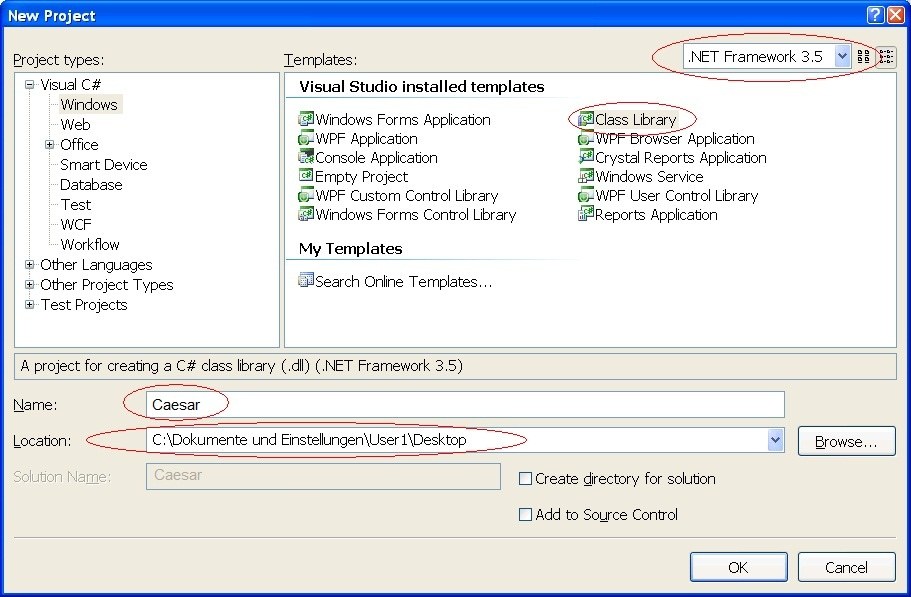
\includegraphics[width=1.00\textwidth]{figures/vs_create_new_project.jpg}
	\caption{Create New Visual Studio/C\# Express Project}
	\label{fig:vs_create_new_project}
\end{figure}\\
Select ''.NET-Framework 3.5'' as the target framework (the Visual Studio Express edition don't provide this selection because it automatically chooses the actual target framework), and ''Class Library'' as default template to create a DLL file. Give the project a unique and significant name (here: ''Caesar''), and choose a location where to save (the Express edition will ask later for a save location when you close your project or your environment). Select the subdirectory ''CrypPlugins'' from your SVN trunk as location. Finally confirm by pressing the ''OK'' button.
\begin{figure}[h]
	\centering
		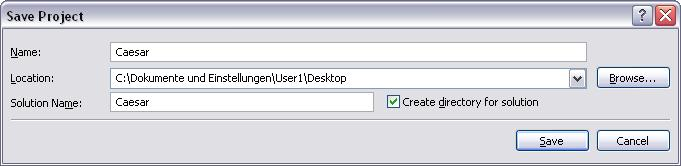
\includegraphics[width=0.80\textwidth]{figures/save_solution_csharp_express.JPG}
	\caption{Microsoft C\# Express Edition save solution dialog}
	\label{fig:save_solution_csharp_express}
\end{figure}\\
Now your Visual Studio/C\# Express solution should look like this:\\
\begin{figure}[h]
	\centering
		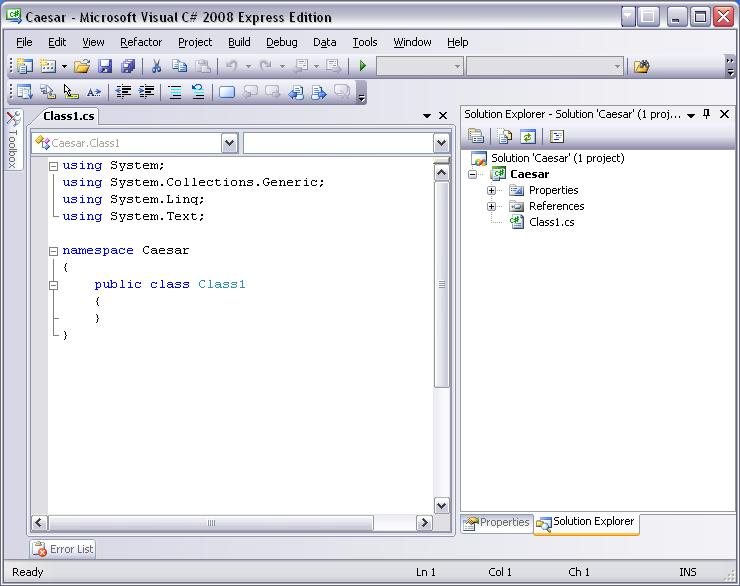
\includegraphics[width=1.00\textwidth]{figures/solution_start_up.jpg}
	\caption{Start-Up solution}
	\label{fig:solution_start_up}
\end{figure}
\section{Interface selection}
\label{sec:SelectTheInterfaceYourPluginWantsToServe}
First we have to add a reference to the CrypTool library called ''CrypPluginBase.dll'' where all necessary CrypTool plugin interfaces are declared.\\
\begin{figure}[h!]
	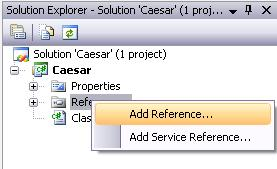
\includegraphics{figures/add_reference.jpg}
	\caption{Add new reference}
	\label{fig:add_reference}
\end{figure}\\
Make a right click in the Solution Explorer on the ''Reference'' item and choose ''Add Reference''.\\
\begin{figure}[h]
	\centering
		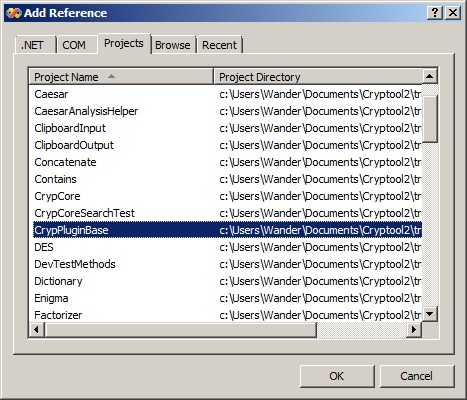
\includegraphics{figures/add_pluginbase_source.jpg}
	\caption{Add reference PluginBase source code}
	\label{fig:add_pluginbase_source}
\end{figure}\\
Select the project ''CrypPluginBase''. If you don't have the CrypPluginBase source code, it's also possible to add a reference the the binary DLL. In this case browse to the path where the library file ''CrypPluginBase.dll'' is located e.g. ''C:\textbackslash Documents and Settings \textbackslash $<$Username$>$ \textbackslash My Documents\textbackslash Visual Studio  2008\textbackslash Projects\textbackslash CrypPluginBase\textbackslash bin\textbackslash Debug'') and select the library by double clicking the file or pressing the "OK" button.\\
\begin{figure}[h]
	\centering
		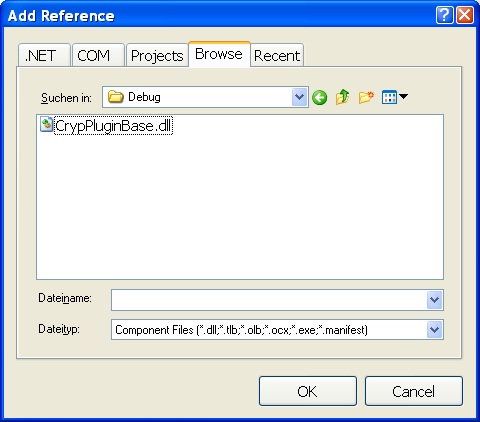
\includegraphics{figures/browse_reference.jpg}
	\caption{Browse reference}
	\label{fig:browse_reference}
\end{figure}\\
Besides the CrypPluginBase you need to add three assembly references (same way like the ''CrypPluginBase'' before by selectig the ''.NET'' tab) to provide the necessary "Windows" namespace for your \textbf{user control} functions called "Presentation" and "QuickWatchPresentation". Select the following .NET components:\\
\begin{itemize}
    \item PresentationCore
    \item PresentationFramework
    \item WindowsBase
\end{itemize}
Afterwards your reference tree view should look like this:
\begin{figure}[h!]
		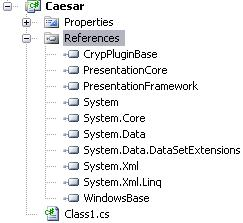
\includegraphics{figures/reference_tree.jpg}
	\caption{Reference tree}
	\label{fig:reference_tree}
\end{figure}
If your plugin will be based on further libraries, you have to add them in the same way.
\section{Create the classes for the algorithm and for its settings}\label{sec:CreateTheClassesForTheAlgorithmAndForItsSettings}
In the next step we have to create two classes. The first class named "Caesar" has to inherit from IEncryption to provide an ecryption plugin. If you want to develop a Hash plugin your class has to inherit from IHash.
The second class named "CaesarSettings" has to inherit from ISettings.
\subsection{Create the class for the algorithm (Caesar)}\label{sec:CreateTheClassForTheAlgorithmCaesar}
Visual Studio automatically creates a class which has the name "Class1.cs".  There are two ways to change the name to "Caesar.cs":
\renewcommand{\labelitemi}{-}
\begin{itemize}
	\item Rename the existent class
	\item Delete the existent class and create a new one.
\end{itemize}
Which one you choose is up to you. We choose the second way as you can see in the next screenshot:
\begin{figure}[h!]
	\centering
		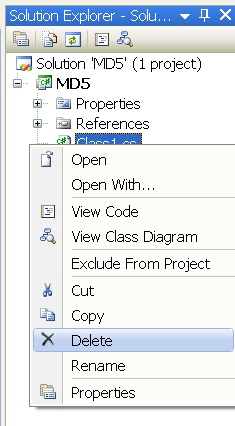
\includegraphics{figures/new_class.jpg}
	\caption{Create new class}
	\label{fig:new_class}
\end{figure}\\
Now make a right click on the project item "Caesar" and select "Add-$>$Class...":
\begin{figure}[h]
	\centering
		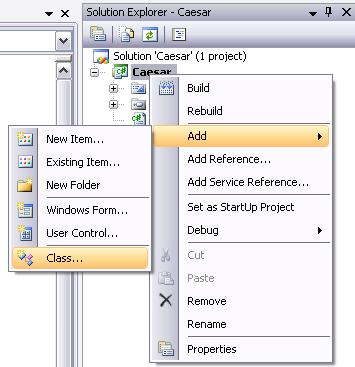
\includegraphics{figures/add_new_class.jpg}
	\caption{Add a new class}
	\label{fig:add_new_class}
\end{figure}\\
Now give your class a unique name. We call the class as mentioned above "Caesar.cs" and make it public to be available to other classes.\\
\begin{figure}[h!]
	\centering
		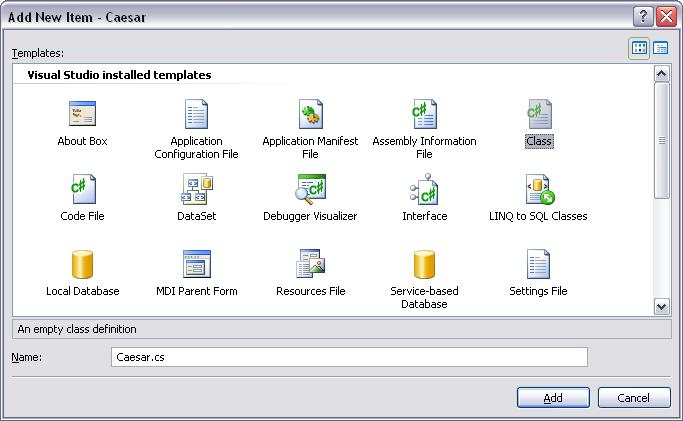
\includegraphics[width=1.00\textwidth]{figures/name_new_class.jpg}
	\caption{Name the new class}
	\label{fig:name_new_class}
\end{figure}\\
\subsection{Create the class for the settings (CaesarSettings)}\label{sec:CreateTheClassForTheSettingsCaesarSettings}
Add a second public class for ISettings in the same way. We call the class "CaesarSettings". The settings class provides the necessary information about controls, captions and descriptions and default parameters for e.g. key settings, alphabets, key length and action to build the \textbf{TaskPane} in CrypTool. How a \textbf{TaskPane} could look like you can see below for the example of a Caesar encryption.\\
\begin{figure}[h!]
	\centering
		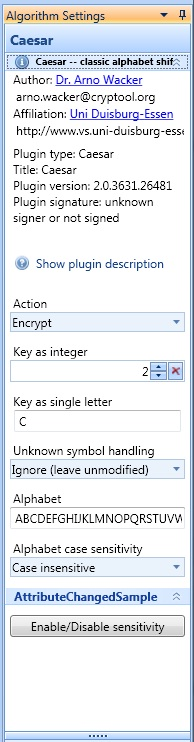
\includegraphics{figures/task_pane.jpg}
	\caption{TaskPane}
	\label{fig:task_pane}
\end{figure}\\
\subsection{Add namespace for the class Caesar and the place from where to inherit}
\label{sec:AddNamespaceForTheClassCaesarAndThePlaceFromWhereToInherit}
Now open the ''Caesar.cs'' file by double clicking on it at the Solution Explorer and include the necessary namespaces to the class header by typing in the according ''using'' statement. The CrypTool 2.0 API provides the following namespaces:
\begin{itemize}
	\item Cryptool.PluginBase = interfaces like IPlugin, IHash, ISettings, attributes, enumerations, delegates and extensions.
	\item Cryptool.PluginBase.Analysis = interface for the crypto analysis plugins like ''Stream Comparator''
	\item Cryptool.PluginBase.Control = ?
	\item Cryptool.PluginBase.Cryptography = interface for all encryption and hash algorithms like AES, DES or MD5 hash
	\item Cryptool.PluginBase.Editor = interface for editors you want to implement for CrypTool 2.0 like the default editor
	\item Cryptool.PluginBase.Generator = interface for generators like the random input generator
	\item Cryptool.PluginBase.IO = interface for CryptoolStream, input and output plugins like text input, file input, text output and file output
	\item Cryptool.PluginBase.Miscellaneous = provides all event helper like GuiLogMessage or PropertyChanged
	\item Cryptool.PluginBase.Resources = ?
	\item Cryptool.PluginBase.Tool = interface for all foreign tools which CrypTool 2.0 has to provide and which does not exactly support the CrypTool 2.0 API
	\item Cryptool.PluginBase.Validation = interface which provides method for validation like regular expression
\end{itemize}
In this case we want to implement a Caesar algorithm which means we need to include the following namespaces:
\begin{itemize}
	\item ''Cryptool.PluginBase'' to provide ''ISettings'' for the CaesarSettings class
	\item ''Cryptool.PluginBase.Cryptography'' to provide ''IEncryption'' for the Caesar class
	\item ''Cryptool.PluginBase.IO'' to provide CryptoolStream for the input and output Data
	\item ''Cryptool.PluginBase.Miscellaneous'' to use the entire CrypTool event handler
\end{itemize}
It is important to define a new default namespace of our public class (''Caesar''). In CrypTool the default namespace is presented by ''Cryptool.[name of class]''. Therefore our namespace has to be defined as follows: ''Cryptool.Caesar''.\\
Up to now the source code should look as you can see below:
\begin{lstlisting}
using System.Collections.Generic;
using System.Text;

//needed CrypTool namespaces
using Cryptool.PluginBase;
using Cryptool.PluginBase.Cryptography;
using Cryptool.PluginBase.IO;
using Cryptool.PluginBase.Miscellaneous;

namespace Cryptool.Caesar
{
	public class Caesar
	{
	}
}
\end{lstlisting}
Next let your class ''Caesar'' inherit from IEncryption by inserting of the following statement:
\begin{lstlisting}
namespace Cryptool.Caesar
{
	public class Caesar: IEncryption
	{
	}
}
\end{lstlisting}
\subsection{Add the interface functions for the class Caesar}\label{sec:AddTheInterfaceFunctionsForTheClassCaesar}
There is an underscore at the ''I'' in IEncryption statement. Move your mouse over it or place the cursor at it and press ''Shift+Alt+F10'' and you will see the following submenu:
\begin{figure}[h!]
	\centering
		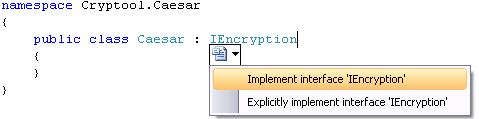
\includegraphics{figures/inherit_submenu.jpg}
	\caption{Inherit submenu}
	\label{fig:inherit_submenu}
\end{figure}\\
Choose the item ''Implement interface 'IEncryption'''. Visual Studio/C\# Express will now place all available and needed interface members to interact with the CrypTool core (this saves you also a lot of typing code).\\
Your code will now look like this:
\begin{lstlisting}
using System.Collections.Generic;
using System.Text;

using Cryptool.PluginBase;
using Cryptool.PluginBase.Cryptography;
using Cryptool.PluginBase.IO;
using Cryptool.PluginBase.Miscellaneous;

namespace Cryptool.Caesar
{
    public class Caesar : IEncryption
    {
        #region IPlugin Members

        public void Dispose()
        {
            throw new NotImplementedException();
        }

        public void Execute()
        {
            throw new NotImplementedException();
        }

        public void Initialize()
        {
            throw new NotImplementedException();
        }

        public event GuiLogNotificationEventHandler OnGuiLogNotificationOccured;

        public event PluginProgressChangedEventHandler OnPluginProgressChanged;

        public event StatusChangedEventHandler OnPluginStatusChanged;

        public void Pause()
        {
            throw new NotImplementedException();
        }

        public void PostExecution()
        {
            throw new NotImplementedException();
        }

        public void PreExecution()
        {
            throw new NotImplementedException();
        }

        public System.Windows.Controls.UserControl Presentation
        {
            get { throw new NotImplementedException(); }
        }

        public System.Windows.Controls.UserControl QuickWatchPresentation
        {
            get { throw new NotImplementedException(); }
        }

        public ISettings Settings
        {
            get { throw new NotImplementedException(); }
        }

        public void Stop()
        {
            throw new NotImplementedException();
        }

        #endregion

        #region INotifyPropertyChanged Members

        public event System.ComponentModel.PropertyChangedEventHandler PropertyChanged;

        #endregion
    }
}
\end{lstlisting}
\subsection{Add namespace and interfaces for the class CaesarSettings}\label{sec:AddNamespaceAndInterfacesForTheClassCaesarSettings}
Let's now take a look at the second class "CaesarSettings" by double clicking at the "CaesarSettings.cs" file at the Solution Explorer. First we also have to include the namespace of "Cryptool.PluginBase" to the class header and let the settings class inherit from "ISettings" analogous as seen before at the Caesar class. Visual Studio/C\# Express will here also automatically place code from the CrypTool interface if available.
\begin{lstlisting}
using System.Collections.Generic;
using System.Text;

using Cryptool.PluginBase;

namespace Cryptool.Caesar
{
    public class CaesarSettings : ISettings
    {
        #region ISettings Members

        public bool HasChanges
        {
            get
            {
                throw new NotImplementedException();
            }
            set
            {
                throw new NotImplementedException();
            }
        }

        #endregion

        #region INotifyPropertyChanged Members

        public event System.ComponentModel.PropertyChangedEventHandler PropertyChanged;

        #endregion
    }
}
\end{lstlisting}
\subsection{Add controls for the class CaesarSettings (if needed)}\label{sec:AddControlsForTheClassCaesarSettingsIfNeeded}
Now we have to implement some kind of controls (like button, text box) if we need them in the CrypTool \textbf{TaskPane} to modify settings of the algorithm. If you decided to provide an algorithm (e.g. Hash) which do not have any kind of settings you can leave this class now empty. The only part you have to modify is the ''HasChanges'' property to avoid any ''NotImplementedException''. How to modify this property you can see in the following code which demonstrate the modifications fot the TaskPane for our Caesar algorithm. You can also take a look at the other algorithm source codes which are stored in our subversion how you can provide a TaskPane. The following source code demonstrates how we provide our TaskPane as seen above.
\begin{lstlisting}
using System;
using System.ComponentModel;
using System.Windows;
using Cryptool.PluginBase;
using System.Windows.Controls;

namespace Cryptool.Caesar
{
    public class CaesarSettings : ISettings
    {
        #region Public Caesar specific interface
        
        /// <summary>
        /// We use this delegate to send log messages from the settings class to the Caesar plugin
        /// </summary>
        public delegate void CaesarLogMessage(string msg, NotificationLevel loglevel);

        /// <summary>
        /// An enumaration for the different modes of dealing with unknown characters
        /// </summary>
        public enum UnknownSymbolHandlingMode { Ignore = 0, Remove = 1, Replace = 2 };

        /// <summary>
        /// Fire if a new status message was send
        /// </summary>
        public event CaesarLogMessage LogMessage;

        public delegate void CaesarReExecute();

        public event CaesarReExecute ReExecute;

        /// <summary>
        /// Retrieves the current sihft value of Caesar (i.e. the key), or sets it
        /// </summary>
        [PropertySaveOrder(0)]
        public int ShiftKey
        {
            get { return shiftValue; }
            set
            {
                setKeyByValue(value);
            }
        }

        /// <summary>
        /// Retrieves the current setting whether the alphabet should be treated as case sensitive or not
        /// </summary>
        [PropertySaveOrder(1)]
        public bool CaseSensitiveAlphabet
        {
            get
            {
                if (caseSensitiveAlphabet == 0)
                {   return false;   }
                else
                {   return true;    }
            }
            set {} // readonly, because there are some problems if we omit the set part.
        }


        /// <summary>
        /// Returns true if some settings have been changed. This value should be set externally to false e.g.
        /// when a project was saved.
        /// </summary>
        [PropertySaveOrder(3)]
        public bool HasChanges
        {
            get { return hasChanges; }
            set { hasChanges = value; }
        }

        #endregion

        #region Private variables
        private bool hasChanges;
        private int selectedAction = 0;
        private string upperAlphabet = ''ABCDEFGHIJKLMNOPQRSTUVWXYZ'';
        private string lowerAlphabet = ''abcdefghijklmnopqrstuvwxyz'';
        private string alphabet = ''ABCDEFGHIJKLMNOPQRSTUVWXYZ'';
        private char shiftChar = 'C';
        private int shiftValue = 2; 
        // private int shiftValue = 2;
        private UnknownSymbolHandlingMode unknownSymbolHandling = UnknownSymbolHandlingMode.Ignore;
        private int caseSensitiveAlphabet = 0; // 0 = case insensitve, 1 = case sensitive
        private bool sensitivityEnabled = true;
        #endregion

        #region Private methods

        private string removeEqualChars(string value)
        {
            int length = value.Length;

            for (int i = 0; i < length; i++)
            {
                for (int j = i + 1; j < length; j++)
                {
                    if ((value[i] == value[j]) || (!CaseSensitiveAlphabet & (char.ToUpper(value[i]) == char.ToUpper(value[j]))))
                    {
                        LogMessage(''Removing duplicate letter: \''' + value[j] + ''\' from alphabet!'', NotificationLevel.Warning);
                        value = value.Remove(j,1);
                        j--;
                        length--;
                    }
                }
            }

            return value;
        }

        /// <summary>
        /// Set the new shiftValue and the new shiftCharacter to offset % alphabet.Length
        /// </summary>
        private void setKeyByValue(int offset)
        {
            HasChanges = true;

            // making sure the shift value lies within the alphabet range      
            offset = offset % alphabet.Length;

            // set the new shiftChar
            shiftChar = alphabet[offset];

            // set the new shiftValue
            shiftValue = offset;

            // Anounnce this to the settings pane
            OnPropertyChanged(''ShiftValue'');
            OnPropertyChanged(''ShiftChar'');

            // print some info in the log.
            LogMessage(''Accepted new shift value '' + offset + ''! (Adjusted shift character to \''' + shiftChar + ''\')'', NotificationLevel.Info);
        }

        private void setKeyByCharacter(string value)
        {
            try
            {
                int offset;
                if (this.CaseSensitiveAlphabet)
                {
                    offset = alphabet.IndexOf(value[0]);
                }
                else
                {
                    offset = alphabet.ToUpper().IndexOf(char.ToUpper(value[0]));
                }
                
                if (offset >= 0)
                {
                    HasChanges = true;
                    shiftValue = offset;
                    shiftChar = alphabet[shiftValue];
                    LogMessage(''Accepted new shift character \''' + shiftChar + ''\'! (Adjusted shift value to '' + shiftValue + '')'', NotificationLevel.Info);
                    OnPropertyChanged(''ShiftValue'');
                    OnPropertyChanged(''ShiftChar'');
                }
                else
                {
                    LogMessage(''Bad input \'''' + value + ''\''! (Character not in alphabet!) Reverting to '' + shiftChar.ToString() + ''!'', NotificationLevel.Error);
                }
            }
            catch (Exception e)
            {
                LogMessage(''Bad input \'''' + value + ''\''! ('' + e.Message + '') Reverting to '' + shiftChar.ToString() + ''!'', NotificationLevel.Error);
            }
        } 

        #endregion

        #region Algorithm settings properties (visible in the Settings pane)

        [PropertySaveOrder(4)]
        [ContextMenu(''Action'', ''Select the Algorithm action'', 1, DisplayLevel.Beginner, ContextMenuControlType.ComboBox, new int[] { 1, 2 }, ''Encrypt'', ''Decrypt'')]
        [TaskPane(''Action'', ''setAlgorithmActionDescription'', null, 1, true, DisplayLevel.Beginner, ControlType.ComboBox, new string[] { ''Encrypt'', ''Decrypt'' })]
        public int Action
        {
            get
            {
                return this.selectedAction;
            }
            set
            {
                if (value != selectedAction) HasChanges = true;
                this.selectedAction = value;
                OnPropertyChanged(''Action'');

                if (ReExecute != null) ReExecute();
            }
        }
        
        [PropertySaveOrder(5)]
        [TaskPane(''Key as integer'', ''Enter the number of letters to shift. For instance a value of 1 means that the plaintext character a gets mapped to the ciphertext character B, b to C and so on.'', null, 2, true, DisplayLevel.Beginner, ControlType.NumericUpDown, ValidationType.RangeInteger, 0, 100)]        
        public int ShiftValue
        {
            get { return shiftValue; }
            set
            {
                setKeyByValue(value);
                if (ReExecute != null) ReExecute();
            }
        }


        [PropertySaveOrder(6)]
        [TaskPaneAttribute(''Key as single letter'', ''Enter a single letter as the key. This letter is mapped to an integer stating the position in the alphabet. The values for \''Key as integer\'' and \''Key as single letter� are always synchronized.'', null, 3, true, DisplayLevel.Beginner, ControlType.TextBox, ValidationType.RegEx, ''^([A-Z]|[a-z]){1,1}'')]
        public string ShiftChar
        {
            get { return this.shiftChar.ToString(); }
            set
            {
                setKeyByCharacter(value);
                if (ReExecute != null) ReExecute();
            }
        }

        [PropertySaveOrder(7)]
        [ContextMenu(''Unknown symbol handling'', ''What should be done with encountered characters at the input which are not in the alphabet?'', 4, DisplayLevel.Expert, ContextMenuControlType.ComboBox, null, new string[] { ''Ignore (leave unmodified)'', ''Remove'', ''Replace with \'?\''' })]
        [TaskPane(''Unknown symbol handling'', ''What should be done with encountered characters at the input which are not in the alphabet?'', null, 4, true, DisplayLevel.Expert, ControlType.ComboBox, new string[] { ''Ignore (leave unmodified)'', ''Remove'', ''Replace with \'?\''' })]
        public int UnknownSymbolHandling
        {
            get { return (int)this.unknownSymbolHandling; }
            set
            {
                if ((UnknownSymbolHandlingMode)value != unknownSymbolHandling) HasChanges = true;
                this.unknownSymbolHandling = (UnknownSymbolHandlingMode)value;
                OnPropertyChanged(''UnknownSymbolHandling'');

                if (ReExecute != null) ReExecute();
            }
        }

        [SettingsFormat(0, ''Normal'', ''Normal'', ''Black'', ''White'', Orientation.Vertical)]
        [PropertySaveOrder(9)]
        [TaskPane(''Alphabet'', ''This is the used alphabet.'', null, 6, true, DisplayLevel.Expert, ControlType.TextBox, '''')]
        public string AlphabetSymbols
        {
          get { return this.alphabet; }
          set
          {
            string a = removeEqualChars(value);
            if (a.Length == 0) // cannot accept empty alphabets
            {
              LogMessage(''Ignoring empty alphabet from user! Using previous alphabet: \'''' + alphabet + ''\'' ('' + alphabet.Length.ToString() + '' Symbols)'', NotificationLevel.Info);
            }
            else if (!alphabet.Equals(a))
            {
              HasChanges = true;
              this.alphabet = a;
              setKeyByValue(shiftValue); //re-evaluate if the shiftvalue is still within the range
              LogMessage(''Accepted new alphabet from user: \'''' + alphabet + ''\'' ('' + alphabet.Length.ToString() + '' Symbols)'', NotificationLevel.Info);
              OnPropertyChanged(''AlphabetSymbols'');

              if (ReExecute != null) ReExecute();
            }
          }
        }

        /// <summary>
        /// Visible setting how to deal with alphabet case. 0 = case insentive, 1 = case sensitive
        /// </summary>   
        //[SettingsFormat(1, ''Normal'')]
        [PropertySaveOrder(8)]
        [ContextMenu(''Alphabet case sensitivity'', ''Should upper and lower case be treated differently? (Should a == A)'', 7, DisplayLevel.Expert, ContextMenuControlType.ComboBox, null, new string[] { ''Case insensitive'', ''Case sensitive'' })]
        [TaskPane(''Alphabet case sensitivity'', ''Should upper and lower case be treated differently? (Should a == A)'', null, 7, true, DisplayLevel.Expert, ControlType.ComboBox, new string[] { ''Case insensitive'', ''Case sensitive'' })]
        public int AlphabetCase
        {
            get { return this.caseSensitiveAlphabet; }
            set
            {
                if (value != caseSensitiveAlphabet) HasChanges = true;
                this.caseSensitiveAlphabet = value;
                if (value == 0)
                {
                    if (alphabet == (upperAlphabet + lowerAlphabet))
                    {
                        alphabet = upperAlphabet;
                        LogMessage(''Changing alphabet to: \'''' + alphabet + ''\'' ('' + alphabet.Length.ToString() + '' Symbols)'', NotificationLevel.Info);
                        OnPropertyChanged(''AlphabetSymbols'');                        
                        // re-set also the key (shiftvalue/shiftChar to be in the range of the new alphabet
                        setKeyByValue(shiftValue);
                    }
                }
                else
                {
                    if (alphabet == upperAlphabet)
                    {
                        alphabet = upperAlphabet + lowerAlphabet;
                        LogMessage(''Changing alphabet to: \'''' + alphabet + ''\'' ('' + alphabet.Length.ToString() + '' Symbols)'', NotificationLevel.Info);
                        OnPropertyChanged(''AlphabetSymbols'');                        
                    }
                }

                // remove equal characters from the current alphabet
                string a = alphabet;
                alphabet = removeEqualChars(alphabet);

                if (a != alphabet)
                {
                    OnPropertyChanged(''AlphabetSymbols'');
                    LogMessage(''Changing alphabet to: \'''' + alphabet + ''\'' ('' + alphabet.Length.ToString() + '' Symbols)'', NotificationLevel.Info);
                }

                OnPropertyChanged(''AlphabetCase'');
                if (ReExecute != null) ReExecute();
            }
        }

        #endregion

        #region INotifyPropertyChanged Members

        public event PropertyChangedEventHandler PropertyChanged;

        protected void OnPropertyChanged(string name)
        {          
          if (PropertyChanged != null)
          {
            PropertyChanged(this, new PropertyChangedEventArgs(name));
          }
        }

        #endregion

        #region TaskPaneAttributeChanged-Sample
        /// <summary>
        /// This event is just used here for sample reasons
        /// </summary>
        public event TaskPaneAttributeChangedHandler TaskPaneAttributeChanged;

        [TaskPane(''Enable/Disable sensitivity'', ''This setting is just a sample and shows how to enable / disable a setting.'', ''AttributeChangedSample'', 8, false, DisplayLevel.Beginner, ControlType.Button)]
        public void EnableDisableSesitivity()
        {
          if (TaskPaneAttributeChanged!= null)
          {
            sensitivityEnabled = !sensitivityEnabled;
            if (sensitivityEnabled)
            {              
              TaskPaneAttributeChanged(this, new TaskPaneAttributeChangedEventArgs(new TaskPaneAttribteContainer(''AlphabetCase'', Visibility.Visible)));
            }
            else
            {
              TaskPaneAttributeChanged(this, new TaskPaneAttributeChangedEventArgs(new TaskPaneAttribteContainer(''AlphabetCase'', Visibility.Collapsed)));
            }
          }
        }
        #endregion TaskPaneAttributeChanged-Sample
    }
}
\end{lstlisting}
\section{Select and add an image as icon for the class Caesar}\label{sec:SelectAndAddAnImageAsIconForTheClassCaesar}
Before we go back to the code of the Caesar class, we have to add an icon image to our project, which will be shown in the CrypTool \textbf{ribbon bar} or/and \textbf{navigation pane}. As there is no default, using an icon image is mandatory.\\\\
\textit{\small Note: This will be changed in future. A default icon will be used if no icon image has been provided.}\\\\
For testing purposes you may create a simple black and white PNG image with MS Paint or Paint.NET. As image size you can use 40x40 pixels for example, but as the image will be scaled when required, any size should do it. Place the image file in your project directory or in a subdirectory. Then make a right click on the project item "Caesar" or any subdirectory within the Solution Explorer, and select ''Add-$>$Existing Item...'':
\begin{figure}[h!]
	\centering
		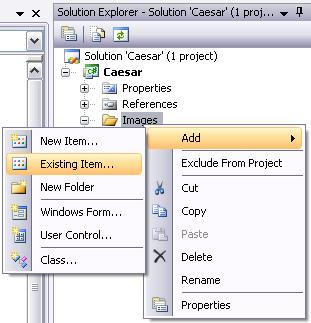
\includegraphics{figures/add_existing_item.jpg}
	\caption{Add existing item}
	\label{fig:add_existing_item}
\end{figure}\\
As you can see, in our solution we create an new folder named ''Images'' (make a right click on the project item ''Caesar'' and select ''Add-$>$New Folder'') and placed there the new icon by clicking right on the folder as mentioned aboved.
Then select ''Image Files'' as file type, and choose the icon for your plugin:
\begin{figure}[h!]
	\centering
		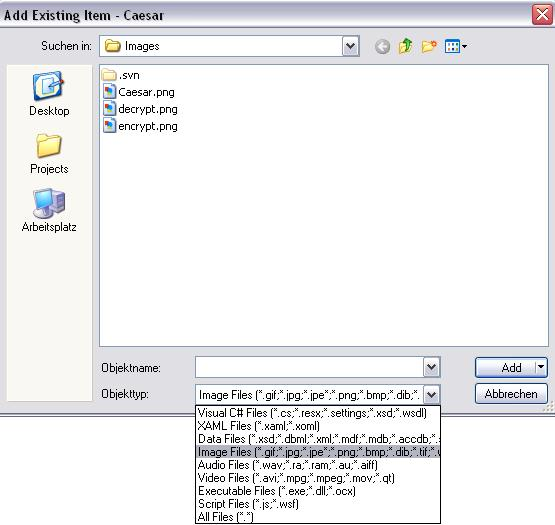
\includegraphics{figures/choose_icon.jpg}
	\caption{Choose the right icon}
	\label{fig:choose_icon}
\end{figure}\\
Finally we have to set the icon as a ''Resource'' to avoid providing the icon as a separate file. Make a right click on the icon and select the item ''Properties'':
\begin{figure}[h!]
	\centering
		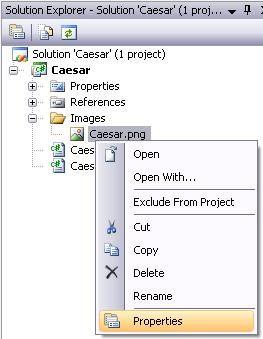
\includegraphics{figures/icon_properties.jpg}
	\caption{Icon properties}
	\label{fig:icon_properties}
\end{figure}\\
In the ''Properties'' panel you have to set the ''Build Action'' to ''Resource'' (not embedded resource):
\begin{figure}[h!]
	\centering
		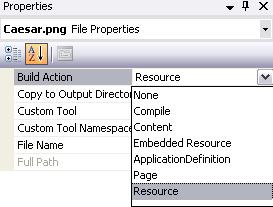
\includegraphics{figures/icon_build_action.jpg}
	\caption{Icon  build action}
	\label{fig:icon_build_action}
\end{figure}
\section{Set the attributes for the class Caesar}\label{sec:SetTheAttributesForTheClassCaesar}
Now let's go back to the code of the Caesar class ("Caesar.cs" file). First we have to set the necessary attributes for our class. This attributes are used to provide additional information for the CrypTool 2.0 environment. If not set, your plugin won't show up in the GUI, even if everything else is implemented correctly.\\\\
Attributes are used for \textbf{declarative} programming and provide meta data, that can be attached to the existing .NET meta data , like classes and properties. Cryptool provides a set of custom attributes, that are used to mark the different parts of your plugin.\\\\
\textit{[Author]}\\
The first attribute called ''Author'' is optional, which means we are not forced to define this attribute. It provides the additional information about the plugin developer. This informations you can see for example in the TaskPane as shown on a screenshot above. We set this attribute to demonstrate how it has to look in case you want to provide this attribute.
\begin{figure}[h!]
	\centering
		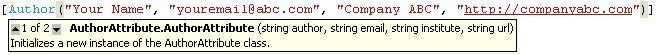
\includegraphics[width=1.00\textwidth]{figures/attribute_author.jpg}
	\caption{Attribute author}
	\label{fig:attribute_author}
\end{figure}\\
As we can see above the author attribute takes four elements of type string. These elements are:
\begin{itemize}
	\item Author = name of the plugin developer
	\item Email = email of the plugin developer if he wants to be contact
	\item Institute = current employment of the developer like University or Company
	\item Url = the website or homepage of the developer
\end{itemize}
All this elements are also optional. The developer decides what he wants to publish. Unused elements shall be set to null or a zero-length string ('''').\\
Our author attribute should look now as you can see below:
\begin{figure}[h!]
	\centering
		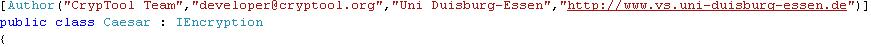
\includegraphics[width=1.00\textwidth]{figures/attribute_author_filled.jpg}
	\caption{Filled author auttribute}
	\label{fig:attribute_author_filled}
\end{figure}\\\\
\textit{[PluginInfo]}\\
The second attribute called ''PluginInfo'' provides the necessary information about the plugin like caption and tool tip. This attribute is mandatory. The attribute has the definition as you can see below:
\begin{figure}[h]
	\centering
		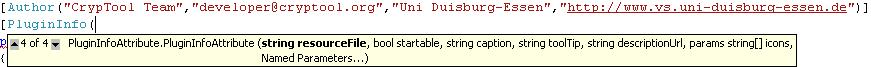
\includegraphics[width=1.00\textwidth]{figures/attribute_plugininfo.jpg}
	\caption{Attribute PluginInfo}
	\label{fig:attribute_plugininfo}
\end{figure}\\
This attribute expects the following elements:
\begin{itemize}
	\item resourceFile = Defines if resource files will be provided and where to find them. E.g. to provide the plugin multilingual you can store the labels in such a resource file. This element is optional.
	\item startable = Set this flag to true only if your plugin is some kind of input or generator plugin (probably if your plugin just has outputs and no inputs). In all other cases use false here. This flag is important. Setting this flag to true for a non input/generator plugin will result in unpredictable chain runs. This element is mandatory.
	\item caption = from type string, the name of the plugin or the resource field name if you provide the caption in a resource file (e.g. to provide the button content). This element is mandatory.
	\item toolTip = from type string, description of the plugin or the resource field name if you provide the toolTip in a resource file (e.g. to provide the button tool tip). This element is optional.
	\item descriptionUrl = from type string, define where to find the whole description files (e.g. XAML files). This element is optional.
	\item icons = from type string array, which provides all necessary icon paths you want to use in the plugin (e.g. the plugin icon as seen above). This element is mandatory.
\end{itemize}
Unused optional elements shall be set to null or a zero-length string ('''').\\\\
\textit{\small Note 1: It is possible to use the plugin without setting a caption though it is not recommended. This will be changed in future and the plugin will fail to load without a caption.\\\\
\small Note 2: Currently a zero-length toolTip string appears as empty box. This will be changed in future.\\\\
\small Note 3: Tooltip and description currently do not support internationalization and localization. This will be changed in future.\\\\}
In our example the first parameter called ''resourceFile'' has to be set to ''Cryptool.Caesar.Resource.res'' because we want to provide the plugin multilingual and want to store the labels and caption in a resource file. Otherwise ignore this element.
\begin{figure}[h]
	\centering
		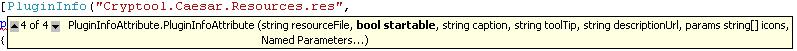
\includegraphics[width=1.00\textwidth]{figures/attribute_plugininfo_resourceFile.JPG}
	\caption{Attribute PluginInfo element resourceFile}
	\label{fig:attribute_plugininfo_resourceFile}
\end{figure}\\
The second parameter called ''startable'' has to be set to ''false'', because our encryption algorithm is neither an input nor generator plugin.
\begin{figure}[h!]
	\centering
		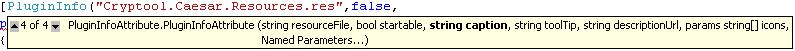
\includegraphics[width=1.00\textwidth]{figures/attribute_plugininfo_startable.jpg}
	\caption{Attribute PluginInfo startable}
	\label{fig:attribute_plugininfo_startable}
\end{figure}\\
The next two parameters are needed to define the plugin's name and its description. Now that we decided to provide a resource file we have to place here the both resource field names which contains the description and captions. Otherwise just write here a simple string text:
\begin{figure}[h!]
	\centering
		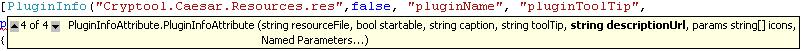
\includegraphics[width=1.00\textwidth]{figures/attribute_plugininfo_description.jpg}
	\caption{Attribute PluginInfo name and description}
	\label{fig:attribute_plugininfo_description}
\end{figure}\\
The next element defines the location path of the description file. The parameter is made up by $<$Assembly name$>$/$<$filename$>$ or $<$Assembly name$>$/$<$Path$>$/$<$file name$>$ if you want to store your description files in a separate folder (as seen on the icon). The description file has to be of type XAML. In our case we create a folder called ''DetailedDescription'' and store our XAML file there with the necessary images if needed. How you manage the files and folders is up to you. This folder could now look as you can see below:
\begin{figure}[h!]
	\centering
		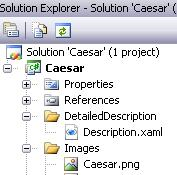
\includegraphics{figures/attribute_plugininfo_detailed_descr_path.jpg}
	\caption{Attribute PluginInfo icon path}
	\label{fig:attribute_plugininfo_icon_path}
\end{figure}\\
Accordingly the attribute parameter has to be set to:
\begin{figure}[h!]
	\centering
		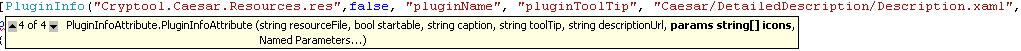
\includegraphics[width=1.00\textwidth]{figures/attribute_plugininfo_detailed_descr.jpg}
	\caption{Attribute PluginInfo icon}
	\label{fig:attribute_plugininfo_icon}
\end{figure}\\
The detailed description could now look like this in CrypTool (right click plugin icon on workspace and select ''Show description''):
\begin{figure}[h]
	\centering
		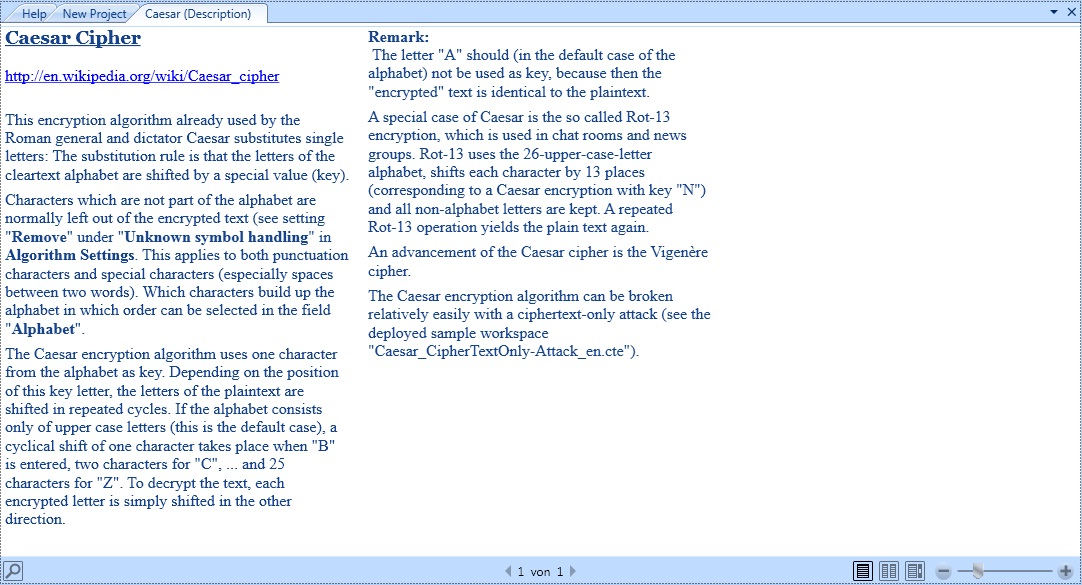
\includegraphics[width=1.00\textwidth]{figures/xaml_description.jpg}
	\caption{XAML detailed description}
	\label{fig:xaml_description}
\end{figure}\\
The last parameter tells CrypTool the names of the provided icons. This parameter is made up by $<$Assembly name$>$/$<$file name$>$ or $<$Assembly name$>$/$<$Path$>$/$<$file name$>$.\\\\
The most important icon is the plugin icon, which will be shown in CrypTool in the ribbon bar or navigation pane (This is the first icon in list, so you have to provide at least one icon for a plugin). As named above how to add an icon to the solution accordingly we have to tell CrypTool where to find the icon by setting this parameter as you can see below:
\begin{figure}[h!]
	\centering
		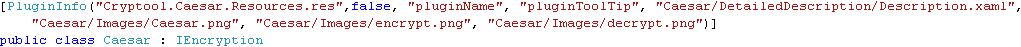
\includegraphics[width=1.00\textwidth]{figures/attribute_plugininfo_icons.jpg}
	\caption{Attribute PluginInfo icons}
	\label{fig:attribute_plugininfo_icons}
\end{figure}\\
You can define further icon paths if needed, by adding the path string separated by a comma. We just add here two further icons (don't forget to add the icons to your solution) to provide them for the context menu in the CrypTool workspace.\\\\
\textit{[EncryptionType]}\\
The third and last attribute called ''EncryptionType'' is needed to tell CrypTool which type of plugin we want to provide. CrypTool is now able to place the plugin in the right group at the navigation pane or/and ribbon bar. Therefore Caesar is a classical algorithm so we have to set the following attribute:
\begin{figure}[h]
	\centering
		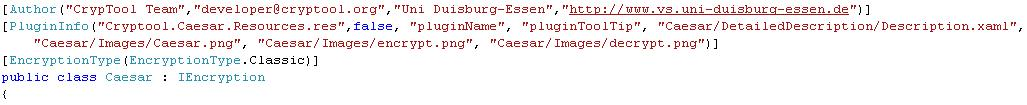
\includegraphics[width=1.00\textwidth]{figures/attribute_encryption_type.JPG}
	\caption{Attribute encryption type}
	\label{fig:attribute_encryption_type}
\end{figure}\\
The ''EncryptionType'' attribute can also be set as the following types:
\begin{itemize}
	\item Asymmetric = for asymmetric encryption algorithms like RSA
	\item Classic = for classic encryption or hash algorithms like Caesar or MD5
	\item Hybrid = for a combination of several algorithm where the data is encrypted symmetric and the encryption key asymmetric
	\item SymmetricBlock = for all block cipher algorithms like DES, AES or Twofish
	\item SymmetricStream = for all stream cipher algorithms like RC4, Rabbit or SEAL
\end{itemize}
\section{Set the private variables for the settings in the class Caesar}\label{sec:SetThePrivateVariablesForTheSettingsInTheClassCaesar}
The next step is to define some private variables needed for the settings, input and output data which could look like this:
\begin{lstlisting}
public class Caesar : IEncryption
{
	#region Private variables
	private CaesarSettings settings;
	private string inputString;
	private string outputString;
	private enum CaesarMode { encrypt, decrypt };
	private List<CryptoolStream> listCryptoolStreamsOut = new List<CryptoolStream>();
	#endregion
\end{lstlisting}
Please notice if there is a sinuous line at the code you type for example at the ''CryptoolStream'' type of the variable listCryptoolStreamsOut. ''CryptoolStream'' is a data type for input and output between plugins and is able to handle large data amounts. To use the CrypTool own stream type, include the namespace ''Cryptool.PluginBase.IO'' with a ''using'' statement as explained in chapter 3.3. Check the other code entries while typing and update the missing namespaces.\\
The following private variables are being used in this example:
\begin{itemize}
	\item CaesarSettings settings: required to implement the IPlugin interface properly
	\item string inputString: sting to read the input data from
	\item string outputString: string to save the output data
	\item enum CaesarMode: our own definition how to select between an encryption or decryption. It's up to you how to solve your algorithm
	\item List$<$CryptoolStream$>$ listCryptoolStreamsOut: list of all streams being created by Caesar plugin, required to perform a clean dispose
\end{itemize}
\section{Define the code of the class Caesar to fit the interface}\label{sec:DefineTheCodeOfTheClassCaesarToFitTheInterface}
Next we have to complete our code to correctly serve the interface.\\
First we add a constructor to our class where we can create an instance of our settings class and a function to handle events:
\begin{lstlisting}
public class Caesar : IEncryption
{
	#region Private variables
	private CaesarSettings settings;
	private string inputString;
	private string outputString;
	private enum CaesarMode { encrypt, decrypt };
	private List<CryptoolStream> listCryptoolStreamsOut = new List<CryptoolStream>();
	#endregion
	
	public Caesar()
	{
		this.settings = new CaesarSettings();
		this.settings.LogMessage += Caesar_LogMessage;
	}
\end{lstlisting}
Secondly, we have to implement the property ''Settings'' defined in the interface:
\begin{lstlisting}
public ISettings Settings
{
	get { return (ISettings)this.settings; }
	set { this.settings = (CaesarSettings)value; }
}
\end{lstlisting}
Thirdly we have to define five properties with their according attributes. This step is necessary to tell Cryptool that these properties are input/output properties used for data exchange with other plugins or to provide our plugin with external data.\\
The attribute is named ''PropertyInfo'' and consists of the following elements:
\begin{itemize}
	\item direction = defines whether this property is an input or output property, i.e. whether it reads input data or writes output data
	\begin{itemize}
		\item Direction.Input
		\item Direction.Output
	\end{itemize}
	\item caption = caption of the property (e.g. shown at the input on the dropped icon in the editor), see below:
\begin{figure}[h]
	\centering
		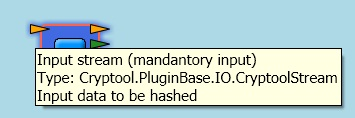
\includegraphics{figures/property_caption.jpg}
	\caption{Possible property caption}
	\label{fig:property_caption}
\end{figure}
	\item toolTip = tooltip of the property (e.g. shown at the input arrow on the dropped icon in the editor), see above
	\item descriptionUrl = not used right now
	\item mandatory = this flag defines whether an input is required to be connected by the user. If set to true, there has to be an input connection that provides data. If no input data is provided for mandatory input, your plugin will not be executed in the workflow chain. If set to false, connecting the input is optional. This only applies to input properties. If using Direction.Output, this flag is ignored.
	\item hasDefaultValue = if this flag is set to true, CrypTool treats this plugin as though the input has already input data.
	\item DisplayLevel = define in which display levels your property will be shown in CrypTool. CrypTool provides the following display levels:
	\begin{itemize}
		\item DisplayLevel.Beginner
		\item DisplayLevel.Experienced
		\item DisplayLevel.Expert
		\item DisplayLevel.Professional
	\end{itemize}
	\item QuickWatchFormat = defines how the content of the property will be shown in the quick watch. CrypTool accepts the following quick watch formats:
	\begin{itemize}
		\item QuickWatchFormat.Base64
		\item QuickWatchFormat.Hex
		\item QuickWatchFormat.None
		\item QuickWatchFormat.Text\\
		A quick watch in Hex could look like this:
\begin{figure}[h]
	\centering
		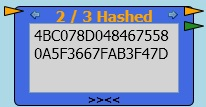
\includegraphics{figures/quick_watch.jpg}
	\caption{Possible quick watch}
	\label{fig:quick_watch}
\end{figure}
	\end{itemize}
	\item quickWatchConversionMethod = this string points to a conversion method; most plugins can use a ''null'' value here, because no conversion is necessary. The QuickWatch function uses system ''default'' encoding to display data. So only if your data is in some other format, like Unicode or UTF8, you have to provide the name of a conversion method as string. The method header has to look like this:
\begin{lstlisting}
object YourMethodName(string PropertyNameToConvert)
\end{lstlisting}
\end{itemize}
First we define the ''InputString'' property getter and setter which is needed to provide our plugin with data which has to be encrypted or decrypted:
\begin{lstlisting}
[PropertyInfo(Direction.InputData, ''Text input'', ''Input a string to be processed by the Caesar cipher'', '''', true, false, DisplayLevel.Beginner, QuickWatchFormat.Text, null)]
public string InputString
{
	get { return this.inputString; }
	set 
  {
		if (value != inputString)
		{
			this.inputString = value;
			OnPropertyChanged(''InputString'');
		}
	}
}
\end{lstlisting}
In the getter we return the value of the input data.\\\\
\textit{\small Note 1: It is currently not possible to read directly from the input data stream without creating an intermediate CryptoolStream.\\\\
\small Note 2: The naming may be confusing. The new CryptoolStream is not an output stream, but it is added to the list of output streams to enable a clean dispose afterwards. See chapter 9 below.\\\\}
The setter checkes if the input value has changed and sets the new input data and announces the data to the CrypTool 2.0 environment by using the expression ''OnPropertyChanged($<$Property name$>$)''. For input properties this step is necessary to update the quick watch view.\\
The output data property (which provides the encrypted or decrypted input data) could look like this:
\begin{lstlisting}
[PropertyInfo(Direction.OutputData, ''Text output'', ''The string after processing with the Caesar cipher'', '''', false, false, DisplayLevel.Beginner, QuickWatchFormat.Text, null)]
public string OutputString
{
	get { return this.outputString; }
	set
	{
		outputString = value;
		OnPropertyChanged(''OutputString'');
	}
}
\end{lstlisting}
CrypTool does not require implementing output setters, as they will never be called from outside of the plugin. Nevertheless in this example our plugin accesses the property itself, therefore we chose to implement the setter.\\
You can also provide additional output data types if you like. For example we provide also an output data of type CryptoolStream, an input data for external alphabets and an input data for the shift value of our Caesar algorithm:
\begin{lstlisting}
[PropertyInfo(Direction.OutputData, ''propStreamOutputToolTip'', ''propStreamOutputDescription'', '''', false, false, DisplayLevel.Beginner, QuickWatchFormat.Text, null)]
public CryptoolStream OutputData
{
	get
	{
		if (outputString != null)
		{                    
			CryptoolStream cs = new CryptoolStream();
			listCryptoolStreamsOut.Add(cs);
			cs.OpenRead(Encoding.Default.GetBytes(outputString.ToCharArray()));
			return cs;
		}
		else
		{
			return null;
		}
	}
	set { }
}

[PropertyInfo(Direction.InputData, ''External alphabet input'', ''Input a string containing the alphabet which should be used by Caesar.\nIf no alphabet is provided on this input, the internal alphabet will be used.'', '''', false, false, DisplayLevel.Expert, QuickWatchFormat.Text, null)]
public string InputAlphabet
{
	get { return ((CaesarSettings)this.settings).AlphabetSymbols; }
	set 
	{
		if (value != null && value != settings.AlphabetSymbols) 
		{ 
			((CaesarSettings)this.settings).AlphabetSymbols = value;
			OnPropertyChanged(''InputAlphabet'');
		} 
	}
}

[PropertyInfo(Direction.InputData, ''Shift value (integer)'', ''Same setting as Shift value in Settings-Pane but as dynamic input.'', '''', false, false, DisplayLevel.Expert, QuickWatchFormat.Text, null)]
public int ShiftKey
{
	get { return settings.ShiftKey; }
	set 
	{ 
		if (value != settings.ShiftKey)
		{
			settings.ShiftKey = value;
		}
	}
}
\end{lstlisting}
This property's setter is not called and therefore not implemented.\\
The CrypTool-API provides two methods to send messages to the CrypTool. The method ''GuiLogMessage'' is used to send messages to the CrypTool status bar. This is a nice feature to inform the user what your plugin is currently doing.
\begin{figure}[h]
	\centering
		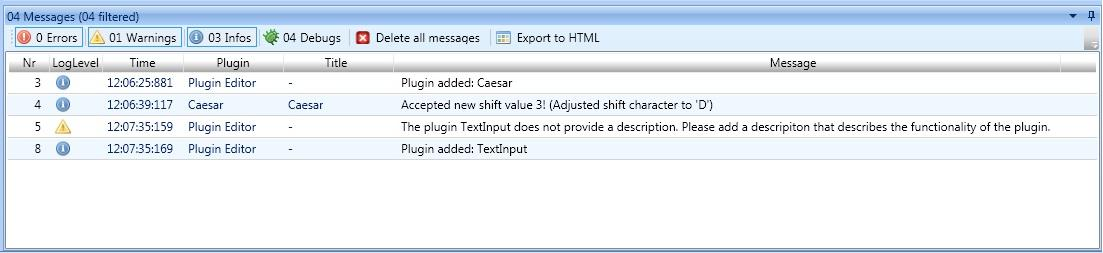
\includegraphics[width=1.00\textwidth]{figures/status_bar.jpg}
	\caption{Status Bar}
	\label{fig:status_bar}
\end{figure}\\
The method takes two parameters which are:
\begin{itemize}
	\item Message = will be shown in the status bar and is of type string
	\item NotificationLevel = to group the messages to their alert level
	\begin{itemize}
		\item NotificationLevel.Error
		\item NotificationLevel.Warning
		\item NotificationLevel.Info
		\item NotificationLevel.Debug
	\end{itemize}
\end{itemize}
As we can recognize we have two methods named ''OnPropertyChanged'' and ''GuiLogMessage'' which are not defined. So we have to define these two methods as you can see below:
\begin{lstlisting}
public event GuiLogNotificationEventHandler OnGuiLogNotificationOccured;
private void GuiLogMessage(string message, NotificationLevel logLevel)
{
	EventsHelper.GuiLogMessage(OnGuiLogNotificationOccured, this, new GuiLogEventArgs(message, this, logLevel));
}

public event PropertyChangedEventHandler PropertyChanged;

public void OnPropertyChanged(String name)
{
	EventsHelper.PropertyChanged(PropertyChanged, this, new PropertyChangedEventArgs(name));
}
\end{lstlisting}
To use the ''PropertyChangedEventHandler'' you have to include the namespace ''System.ComponentModel''.\\
Our whole included namespaces looks now like this:
\begin{lstlisting}
using System.Collections.Generic;
using System.Text;
using System.ComponentModel;
using System.Windows.Control;

using Cryptool.PluginBase;
using Cryptool.PluginBase.Cryptography;
using Cryptool.PluginBase.IO;
using Cryptool.PluginBase.Miscellaneous;
\end{lstlisting}
\section{Complete the actual code for the class Caesar}\label{sec:CompleteTheActualCodeForTheClassCaesar}
Up to now, the plugin is ready for the CrypTool base application to be accepted and been shown correctly in the CrypTool menu. What we need now, is the implementation of the actual algorithm in the function ''Execute()'' which is up to you as the plugin developer. CrypTool will always call first the Execute() function.If you place the whole algorithm in this function or split in other as needed is also up to you.\\
We decided to split our algorithm encryption and decryption in two seperate functions, which finally call the function ProcessCaesar.\\
Let us demonstrate the Execute() function, too:
\begin{lstlisting}
private void ProcessCaesar(CaesarMode mode)
{
	CaesarSettings cfg = (CaesarSettings)this.settings;
	StringBuilder output = new StringBuilder('''');
	string alphabet = cfg.AlphabetSymbols;

  // in case we want don't consider case in the alphabet, we use only capital letters, hence transform 
	// the whole alphabet to uppercase
	if (!cfg.CaseSensitiveAlphabet)
	{
		alphabet = cfg.AlphabetSymbols.ToUpper(); ;
	}
            
	if (inputString != null)
	{
		for (int i = 0; i < inputString.Length; i++)
		{
			// get plaintext char which is currently processed
			char currentchar = inputString[i];

			// remember if it is upper case (otherwise lowercase is assumed)
			bool uppercase = char.IsUpper(currentchar);

			// get the position of the plaintext character in the alphabet
			int ppos = 0;
			if (cfg.CaseSensitiveAlphabet)
			{
				ppos = alphabet.IndexOf(currentchar);
			}
			else
			{
				ppos = alphabet.IndexOf(char.ToUpper(currentchar));
			}

			if (ppos >= 0)
			{
				// we found the plaintext character in the alphabet, hence we do the shifting
				int cpos = 0; ;
				switch (mode)
				{
					case CaesarMode.encrypt:
						cpos = (ppos + cfg.ShiftKey) % alphabet.Length;
						break;
					case CaesarMode.decrypt:
						cpos = (ppos - cfg.ShiftKey + alphabet.Length) % alphabet.Length;
						break;
				}

				// we have the position of the ciphertext character, hence just output it in the correct case
				if (cfg.CaseSensitiveAlphabet)
				{
					output.Append(alphabet[cpos]);
				}
				else
				{
					if (uppercase)
					{
						output.Append(char.ToUpper(alphabet[cpos]));
					}
					else
					{
						output.Append(char.ToLower(alphabet[cpos]));
					}
				}
			}
			else
			{
				// the plaintext character was not found in the alphabet, hence proceed with handling unknown characters
				switch ((CaesarSettings.UnknownSymbolHandlingMode)cfg.UnknownSymbolHandling)
				{
					case CaesarSettings.UnknownSymbolHandlingMode.Ignore:
						output.Append(inputString[i]);
						break;
					case CaesarSettings.UnknownSymbolHandlingMode.Replace:
						output.Append('?');
						break;
				}
			}

			//show the progress
			if (OnPluginProgressChanged != null)
			{
				OnPluginProgressChanged(this, new PluginProgressEventArgs(i, inputString.Length - 1));
			}
		}
		outputString = output.ToString();
		OnPropertyChanged(''OutputString'');
		OnPropertyChanged(''OutputData'');
	}
}

public void Encrypt()
{
	ProcessCaesar(CaesarMode.encrypt);
}

public void Decrypt()
{
	ProcessCaesar(CaesarMode.decrypt);
}

public void Execute()
{
	switch (settings.Action)
	{
		case 0:
			Caesar_LogMessage(''encrypting'', NotificationLevel.Debug);
			Encrypt();
			break;
		case 1:
			Decrypt();
			break;
		default:
    	break;
	}
}
\end{lstlisting}
It is important to make sure that all changes of output properties will be announced to the CrypTool environment. In this example this happens by calling the setter of OutputData which in turn calls ''OnPropertyChanged'' for both output properties ''OutputData'' and ''OutputDataStream''. Instead of calling the property's setter you can as well call ''OnPropertyChanged'' directly within the ''Execute()'' method.\\\\
Certainly you have seen the unknown method ''ProgressChanged'' which you can use to show the current algorithm process as a progress on the plugin icon.
To use this method you also have to declare this method to afford a successful compilation:
\begin{lstlisting}
public event PluginProgressChangedEventHandler OnPluginProgressChanged;
private void ProgressChanged(double value, double max)
{
	EventsHelper.ProgressChanged(OnPluginProgressChanged, this, new PluginProgressEventArgs(value, max));
}
\end{lstlisting}
\section{Perform a clean dispose}\label{sec:PerformACleanDispose}
Be sure you have closed and cleaned all your streams after execution and when CrypTool decides to dispose the plugin instance. Though not required, we run the dispose code before execution as well:
\begin{lstlisting}
public void Dispose()
{
	foreach(CryptoolStream stream in listCryptoolStreamOut)
	{
		stream.Close();
	}
	listCryptoolStreamOut.Clear();
}

public void PostExecution()
{
	Dispose();
}

public void PreExecution()
{
	Dispose();
}
\end{lstlisting}
\section{Finish implementation}\label{sec:FinishImplementation}
When adding plugin instances to the CrypTool workspace, CrypTool checks whether the plugin runs without any exception. If any IPlugin method throws an exception, CrypTool will show an error and prohibit using the plugin. Therefore we have to remove the ''NotImplementedException'' from the methods ''Initialize()'', ''Pause()'' and ''Stop()''. In our example it's sufficient to provide empty implementations.
\begin{lstlisting}
public void Initialize()
{
}

public void Pause()
{
}

public void Stop()
{
}
\end{lstlisting}
The methods ''Presentation()'' and ''QuickWatchPresentation()'' can be used if a plugin developer wants to provide an own visualization of the plugin algorithm which will be shown in CrypTool. Take a look at the PRESENT plugin to see how a custom visualization can be realized. For our Caesar example we don't want to implement a custom visualization, therefore we return ''null'':
\begin{lstlisting}
public UserControl Presentation
{
	get { return null; }
}

public UserControl QuickWatchPresentation
{
	get { return null; }
}
\end{lstlisting}
Your plugin should compile without errors at this point.
\section{Sign the created plugin}\label{sec:SignTheCreatedPlugin}
\section{Import the plugin to Cryptool and test it}\label{sec:ImportThePluginToCryptoolAndTestIt}
After you have built the plugin, you need to move the newly created plugin DLL to a location, where CrypTool can find it. To do this, there are the following ways:
\begin{itemize}
	\item Copy your plugin DLL file in the folder ''CrypPlugins'' which has to be in the same folder as the CrypTool executable, called ''CrypWin.exe''. If necessary, create the folder ''CrypPlugins''.
\begin{figure}[h]
	\centering
		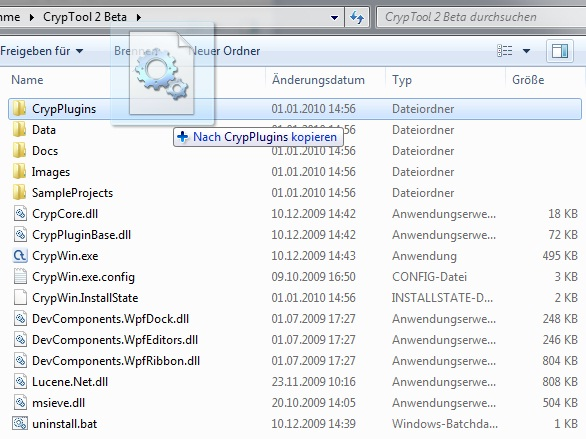
\includegraphics{figures/copy_dll_global_storage.jpg}
	\caption{Copy plugin to global storage}
	\label{fig:copy_dll_global_storage}
\end{figure}\\
This folder is called ''Global storage'' in the CrypTool architecture. Changes in this folder will take effect for all users on a multi user Windows. Finally restart CrypTool.
\begin{figure}[h]
	\centering
		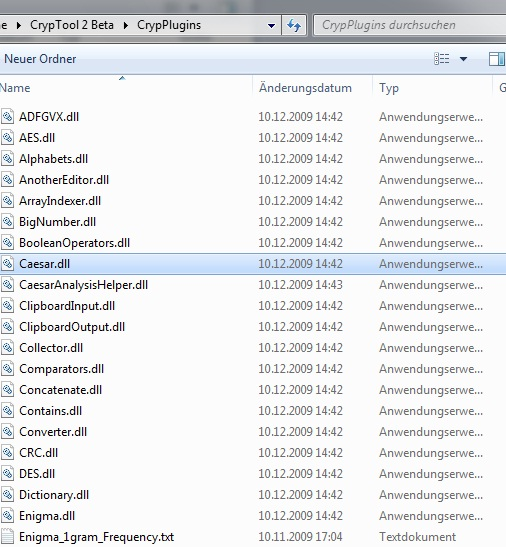
\includegraphics{figures/global_storage.jpg}
	\caption{Plugins global storage}
	\label{fig:global_storage}
\end{figure}\\
	\item Copy your plugin DLL file in the folder ''CrypPlugins'' which is located in your home path in the folder ''ApplicationData'' and restart CrypTool.  This home folder path is called ''Custom storage'' in the CrypTool architecture. Changes in this folder will only take effect for current user.  On a German Windows XP the home folder path could look like:
''C:\textbackslash Dokumente und Einstellungen\textbackslash $<$User$>$\textbackslash Anwendungsdaten\textbackslash CrypPlugins'' and in Vista/Windows7 the path will look like ''C:\textbackslash Users\textbackslash $<$user$>$\textbackslash Application Data\textbackslash CrypPlugins''.
\begin{figure}[h]
	\centering
		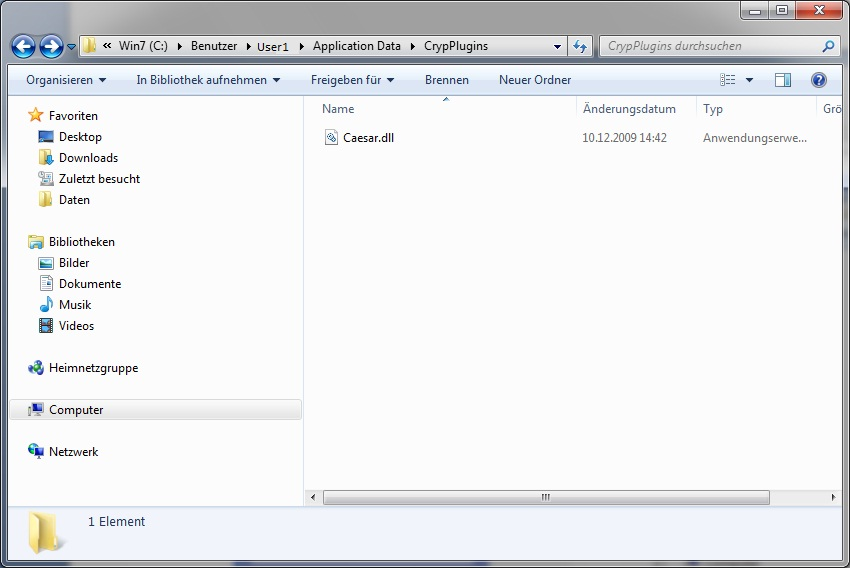
\includegraphics[width=1.00\textwidth]{figures/custom_storage.jpg}
	\caption{Plugins custom storage}
	\label{fig:custom_storage}
\end{figure}
	\item You can also import new plugins directly from the CrypTool interface. Just execute CrypWin.exe and select the ''Download Plugins'' button. An ''Open File Dialog'' will open and ask where the new plugin is located. After selecting the new plugin, CrypTool will automatically import the new plugin in the custom storage folder. With this option you will not have to restart CrypTool. All according menu entries will be updated automatically.
Notice, that this plugin importing function only accepts \textbf{signed} plugins.

\textit{\small Note: This option is a temporary solution for importing new plugins. In the future this will be done online by a web service.}

	\item Use post-build in your project properties to copy the DLL automatically after building it in Visual Studio with other plugins. Right-click on your plugin project and select ''Properties'':
\begin{figure}[h]
	\centering
		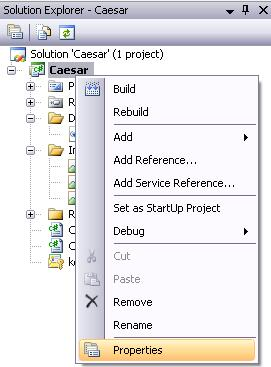
\includegraphics{figures/solution_properties.JPG}
	\caption{Solution Properties}
	\label{fig:solution_properties}
\end{figure}\\
Select ''Build Events'':
\begin{figure}[h]
	\centering
		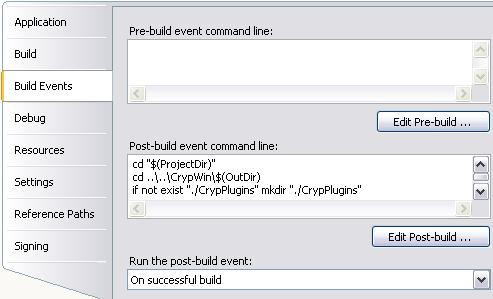
\includegraphics{figures/post_build.JPG}
	\caption{Build Events}
	\label{fig:post_build}
\end{figure}\\
Enter the following text snippet into ''Post-build event command line'':\\\\
cd ''\$(ProjectDir)''\\
cd ..\textbackslash ..\textbackslash CrypWin\$(OutDir)\\
if not exist ''./CrypPlugins'' mkdir ''./CrypPlugins''\\
del /F /S /Q /s /q ''\fcolorbox{yellow}{yellow}{Caesar}*.*''\\
copy ''\$(TargetDir)\fcolorbox{yellow}{yellow}{Caesar}*.*'' ''./CrypPlugins''\\\\
You need to adapt the yellow marked field to your actual project name.
\end{itemize}
\section{Source code and source template}\label{sec:SourceCodeAndSourceTemplate}
Here you can download the whole source code which was presented in this ''Howto'' as a Visual Studio \textbf{solution}:\\\\
\textit{username: anonymous\\
password: not required\\}
\htmladdnormallink{https://www.cryptool.org/svn/CrypTool2/trunk/CrypPlugins/Caesar/}{https://www.cryptool.org/svn/CrypTool2/trunk/CrypPlugins/Caesar/}\\\\
Here you can download the Visual Studio plugin \textbf{template} to begin with the development of a new Cryptool plugin:\\\\
\htmladdnormallink{http://cryptool2.vs.uni-due.de/downloads/template/encryptionplugin.zip}{http://cryptool2.vs.uni-due.de/downloads/template/encryptionplugin.zip}
\section{Provide a workflow file of your plugin}\label{ProvideAWorkflowFileOfYourPlugin}
Every plugin developer should provide a workflow file which shows his algorithm working in CrypTool2. You will automatically create a workflow file by saving your project which was created on CrypTool2 work space. Here is an example how a workflow could look like:
\begin{figure}[h]
	\centering
		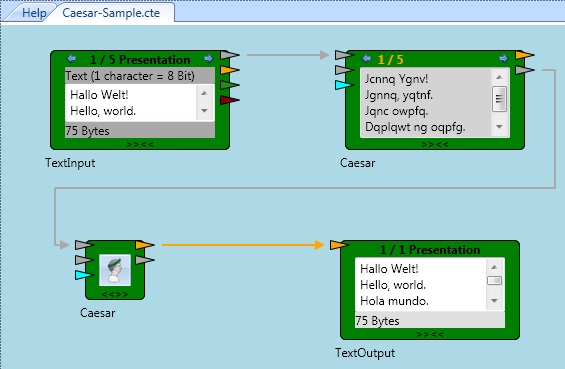
\includegraphics{figures/sample.jpg}
	\caption{Plugin sample}
	\label{fig:sample}
\end{figure}